
This three-dimensional benchmark was first proposed by \cite{bucc93}. 
It has been subsequently presented in \cite{tack94,trha98,albe00,omma06,dawk11,krhb12}.
We here focus on Case 1 of \cite{bucc93}:  an isoviscous bimodal convection experiment at $Ra=3\cdot 10^5$.

The domain is of size $a\times b\times h$ with $a=1.0079h$, $b=0.6283h$ with $h=2700$km. It is filled with a Newtonian fluid characterised by $\rho_0=3300{\rm kg}.{\rm m}^{-3}$, $\alpha=10^{-5}{\rm K}^{-1}$, 
$\mu=8.0198\times10^{23}{\rm Pa.s}$, 
$k=3.564{\rm W}.{\rm m}^{-1}.{\rm K}^{-1}$, 
$c_p=1080{\rm J}.{\rm K}^{-1}.{\rm kg}^{-1}$.
The gravity vector is set to ${\bm g}=(0,0,-10)^T$.
The temperature is imposed at the bottom  ($T=3700^\circ$C) and at the top ($T=0^\circ$C).

Note that using these numbers (as privided in the original paper), we arrive at Ra=29967.01, which 
is not exactly $3\cdot10^5$ as announced. Also, the heat diffusivity $\kappa=k/\rho_0 c_p$ is 
{\it exactly} $10^{-6}$.

The various measurements presented in \cite{bucc93} are listed hereafter:
\begin{itemize}
\item The Nusselt number $Nu$ computed at the top surface following Eq. (\ref{eqNu}):
\[
Nu = L_z \frac{\int\int_{z=L_z} \frac{\partial T}{\partial y} dx dy  }{\int \int_{z=0} T dx dy}
\]
\item the root mean square velocity $v_{rms}$ and the temperature mean square velocity $T_{rms}$
\item The vertical velocity $w$ and temperature $T$ at points ${\bm x}_1=(0,0,L_z/2)$, ${\bm x}_2=(L_x,0,L_z/2)$,
${\bm x}_3=(0,L_y,L_z/2)$ and ${\bm x}_4=(L_x,L_y,L_z/2)$;
\item the vertical component of the heat flux $Q$ at the top surface  at all four corners. OR IS IT TEMP DERIVATIVE?
\end{itemize}

%............................
\subsubsection*{Methodology}

In what follows I highlight a few important points which are key to understanding how the code
is put together and works. 

\begin{verbatim}

load needed modules and functions
define parameters
build V grid (xV,yV,zV)
build V connectivity (iconV)
define b.c. for velocity (bc_fixV,bc_valV)
build T grid (xT,yT,zT)
build T connectivity (iconT)
define b.c. for temperature (bc_fixT,bc_valT)
initial temperature field
.------------------------> istep ---------------------.
|  build K,G,f,h                                      |
|  assemble them in A,rhs                             |
|  solve                                              |
|  split solution vector in u,v,w,p                   |
|  compute dt from CFL condition                      |
|  compute vrms                                       |
|  build A, rhs for temperature                       |
|  solve for temperature T                            |
|  compute elemental strainrate                       |
|  compute nodal strainrate                           |
|  compute nodal pressure                             |
|  measure V and T at mid side edges                  |
|  export to vtu and ascii files                      | 
<-----------------------------------------------------.
\end{verbatim}

I fist load the shape functions which are in two separate files:

\begin{lstlisting}
from shape_functionsV import NNV,dNNVdr,dNNVds,dNNVdt
from shape_functionsT import NNT,dNNTdr,dNNTds,dNNTdt
\end{lstlisting}

There are NV=nnx*nny*nnz velocity nodes and NT=NV temperature nodes.

The velocity grid is built: xV, yV, zV, iconV, and 
these are copied in xT, yT, zT and iconT for the temperature grid.  

The initial temperature field is built as follows:
\begin{lstlisting}
for i in range(0,NT):
   T[i]= (Temperature2-Temperature1)/Lz*zT[i]+Temperature1 \
       + 100*(np.cos(np.pi*xT[i]/Lx) + np.cos(np.pi*yT[i]/Ly))*np.sin(np.pi*zT[i]/Lz)
\end{lstlisting}

The ${\bm C}$ matrix of Eq.~\ref{eq:mixedC} is then built:
\begin{lstlisting}
c_mat = np.array([[2,0,0,0,0,0],\
                  [0,2,0,0,0,0],\
                  [0,0,2,0,0,0],\
                  [0,0,0,1,0,0],\
                  [0,0,0,0,1,0],\
                  [0,0,0,0,0,1]],dtype=np.float64) 
\end{lstlisting}



%.......................
\subsubsection*{Results}

\begin{center}
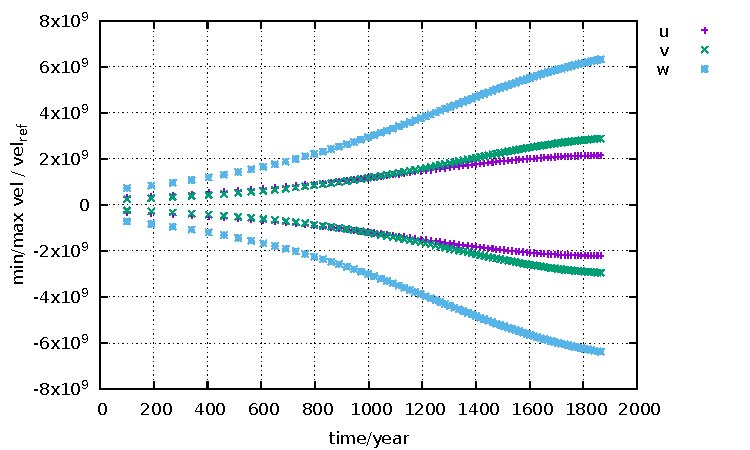
\includegraphics[width=7cm]{python_codes/fieldstone_20/images/velstats.pdf}
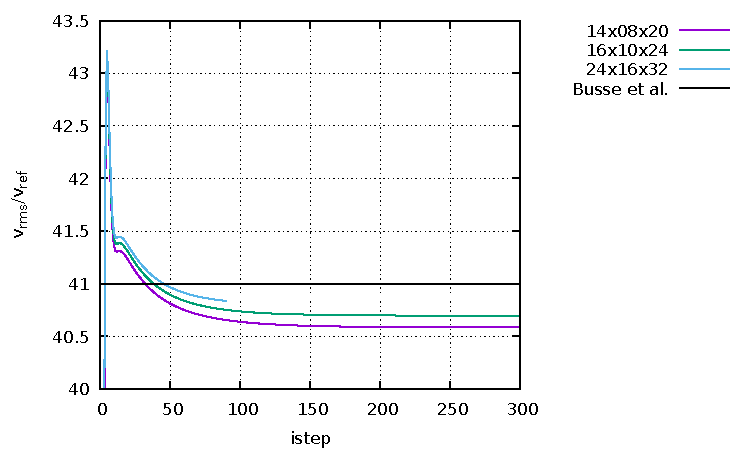
\includegraphics[width=7cm]{python_codes/fieldstone_20/images/vrms.pdf}\\
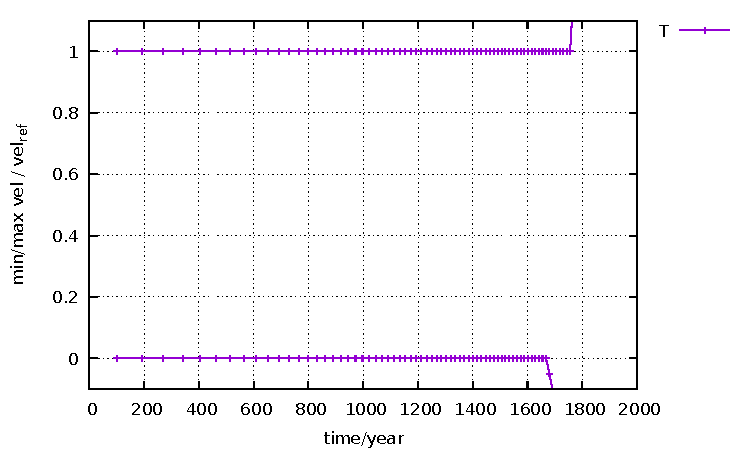
\includegraphics[width=7cm]{python_codes/fieldstone_20/images/Tstats.pdf}
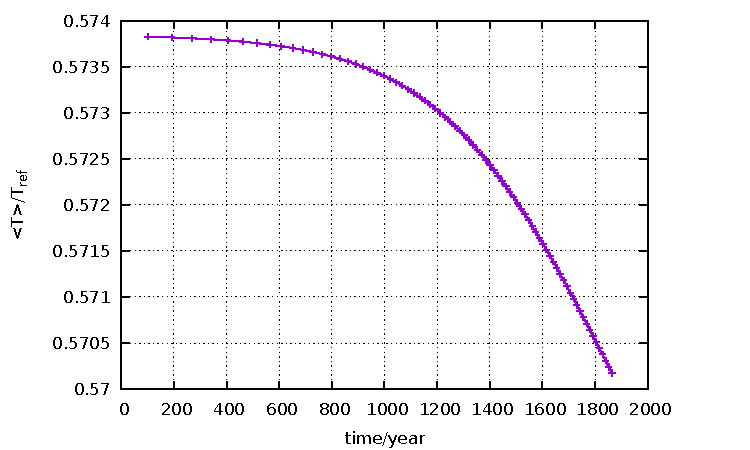
\includegraphics[width=7cm]{python_codes/fieldstone_20/images/Tavrg.pdf}\\
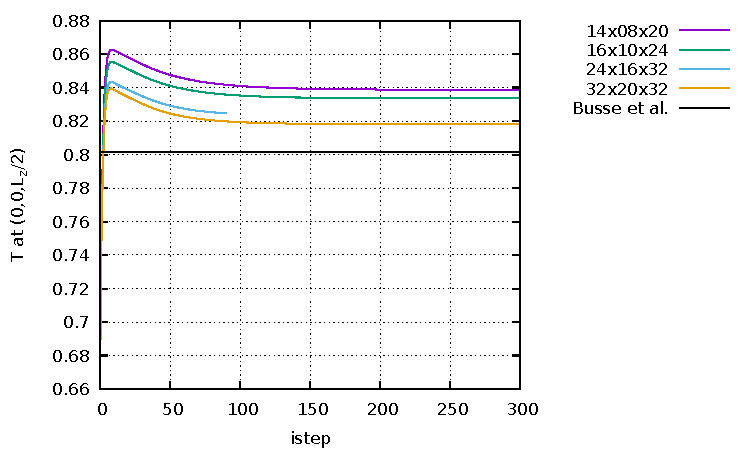
\includegraphics[width=7cm]{python_codes/fieldstone_20/images/Tmid.pdf}
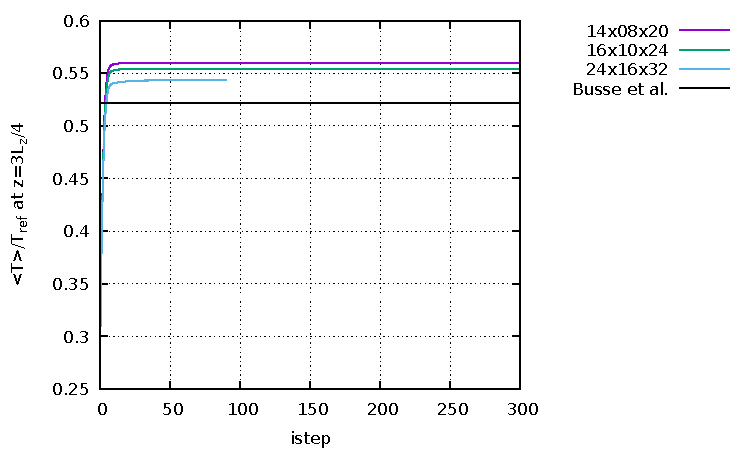
\includegraphics[width=7cm]{python_codes/fieldstone_20/images/Tm.pdf}\\
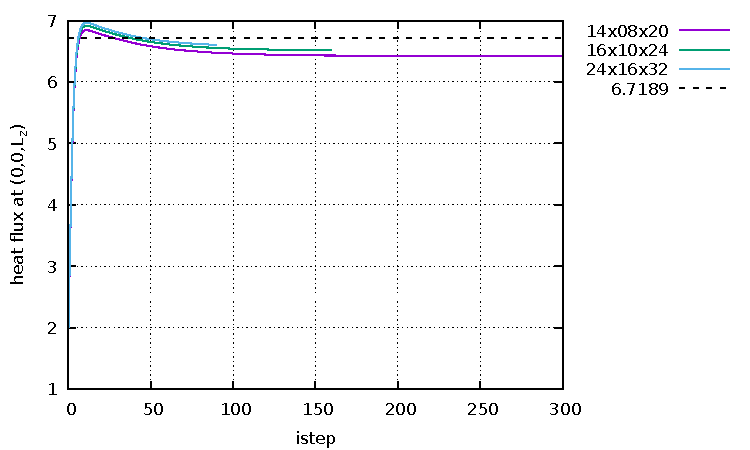
\includegraphics[width=7cm]{python_codes/fieldstone_20/images/hf.pdf}
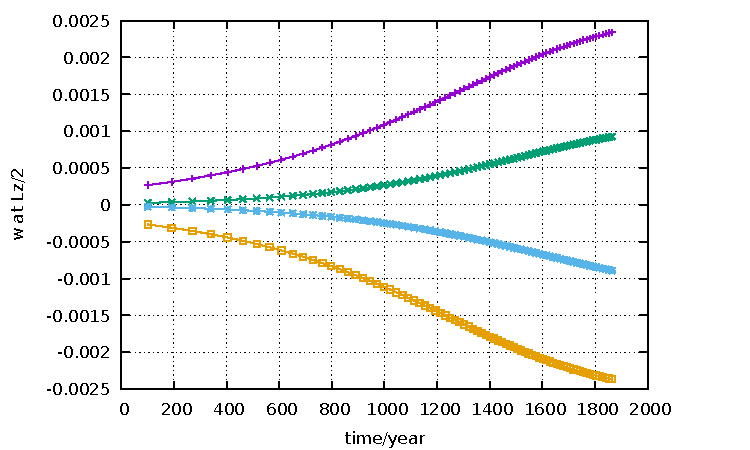
\includegraphics[width=7cm]{python_codes/fieldstone_20/images/wmid.pdf}
\end{center}


The reported values for Busse et al. in the following table are taken from Table 3 of \cite{bucc93}.
The reported values for fieldstone are adimensionalised by means of a reference temperature (3700K),
a reference lengthscale 2700km, and a reference time $L_z^2/\kappa\sim 7.29e+18$s. 
To find the steady state, we simulate the problem up to non-dimensional time $t=5$, 
i.e. $t=3.645e+19$s.



\begin{tabular}{llllll}
\hline
                                & ASPECT &       &       & Busse et al \cite{bucc93} & fieldstone \\
Mesh size                       & Lz/24  & Lz/32 & Lz/48 & (best results)            & 20x12x20    \\
\hline
Nu                              &  & &  & $3.5374  \pm 0.0005$   \\
$v_{rms}$                       &  & &  & $40.999  \pm 0.004$    \\
$\langle T\rangle$ at $0.75*Lz$ &  & &  & $0.52148 \pm 0.00003$  \\
$w(0,0,L_z/2)$     &  &&& $116.625 \pm 0.030$ \\
$w(L_x,0,L_z/2)$   & - &-&-& -\\
$w(L_x,L_y,L_z/2)$ & - &-&-& -\\
$w(0,L_y,L_z/2)$   &  &&& $40.500 \pm 0.030$ \\
$T(0,0,L_z/2)$     &  &&& $0.80130 \pm 0.00005$ \\
$T(L_x,0,L_z/2)$   &  -&-&-& -\\
$T(L_x,L_y,L_z/2)$ &  -&-&-& -\\
$T(0,L_y,L_z/2)$   &  &&& $0.61876 \pm 0.00005$ \\
$dTdz(0,0,L_z)$    &  &&& $6.7127 \pm 0.0500$ \\
$dTdz(L_x,0,L_z)$  &  &&& $1.5080 \pm 0.0500$ \\
$dTdz(L_x,L_y,L_z)$&  &&& $0.7140 \pm 0.0500$ \\
$dTdz(0,L_y,L_z)$  &  &&& $3.1740 \pm 0.0500$ \\
\hline
\end{tabular}




NUSSELT NUMBER !!

